\chapter{Result}
\label{results}
Having a concept on how to translate a rust program into a Petri-Net, we can now inspect the actual results.
\section{Translation target}
\begin{figure}
  \centering
  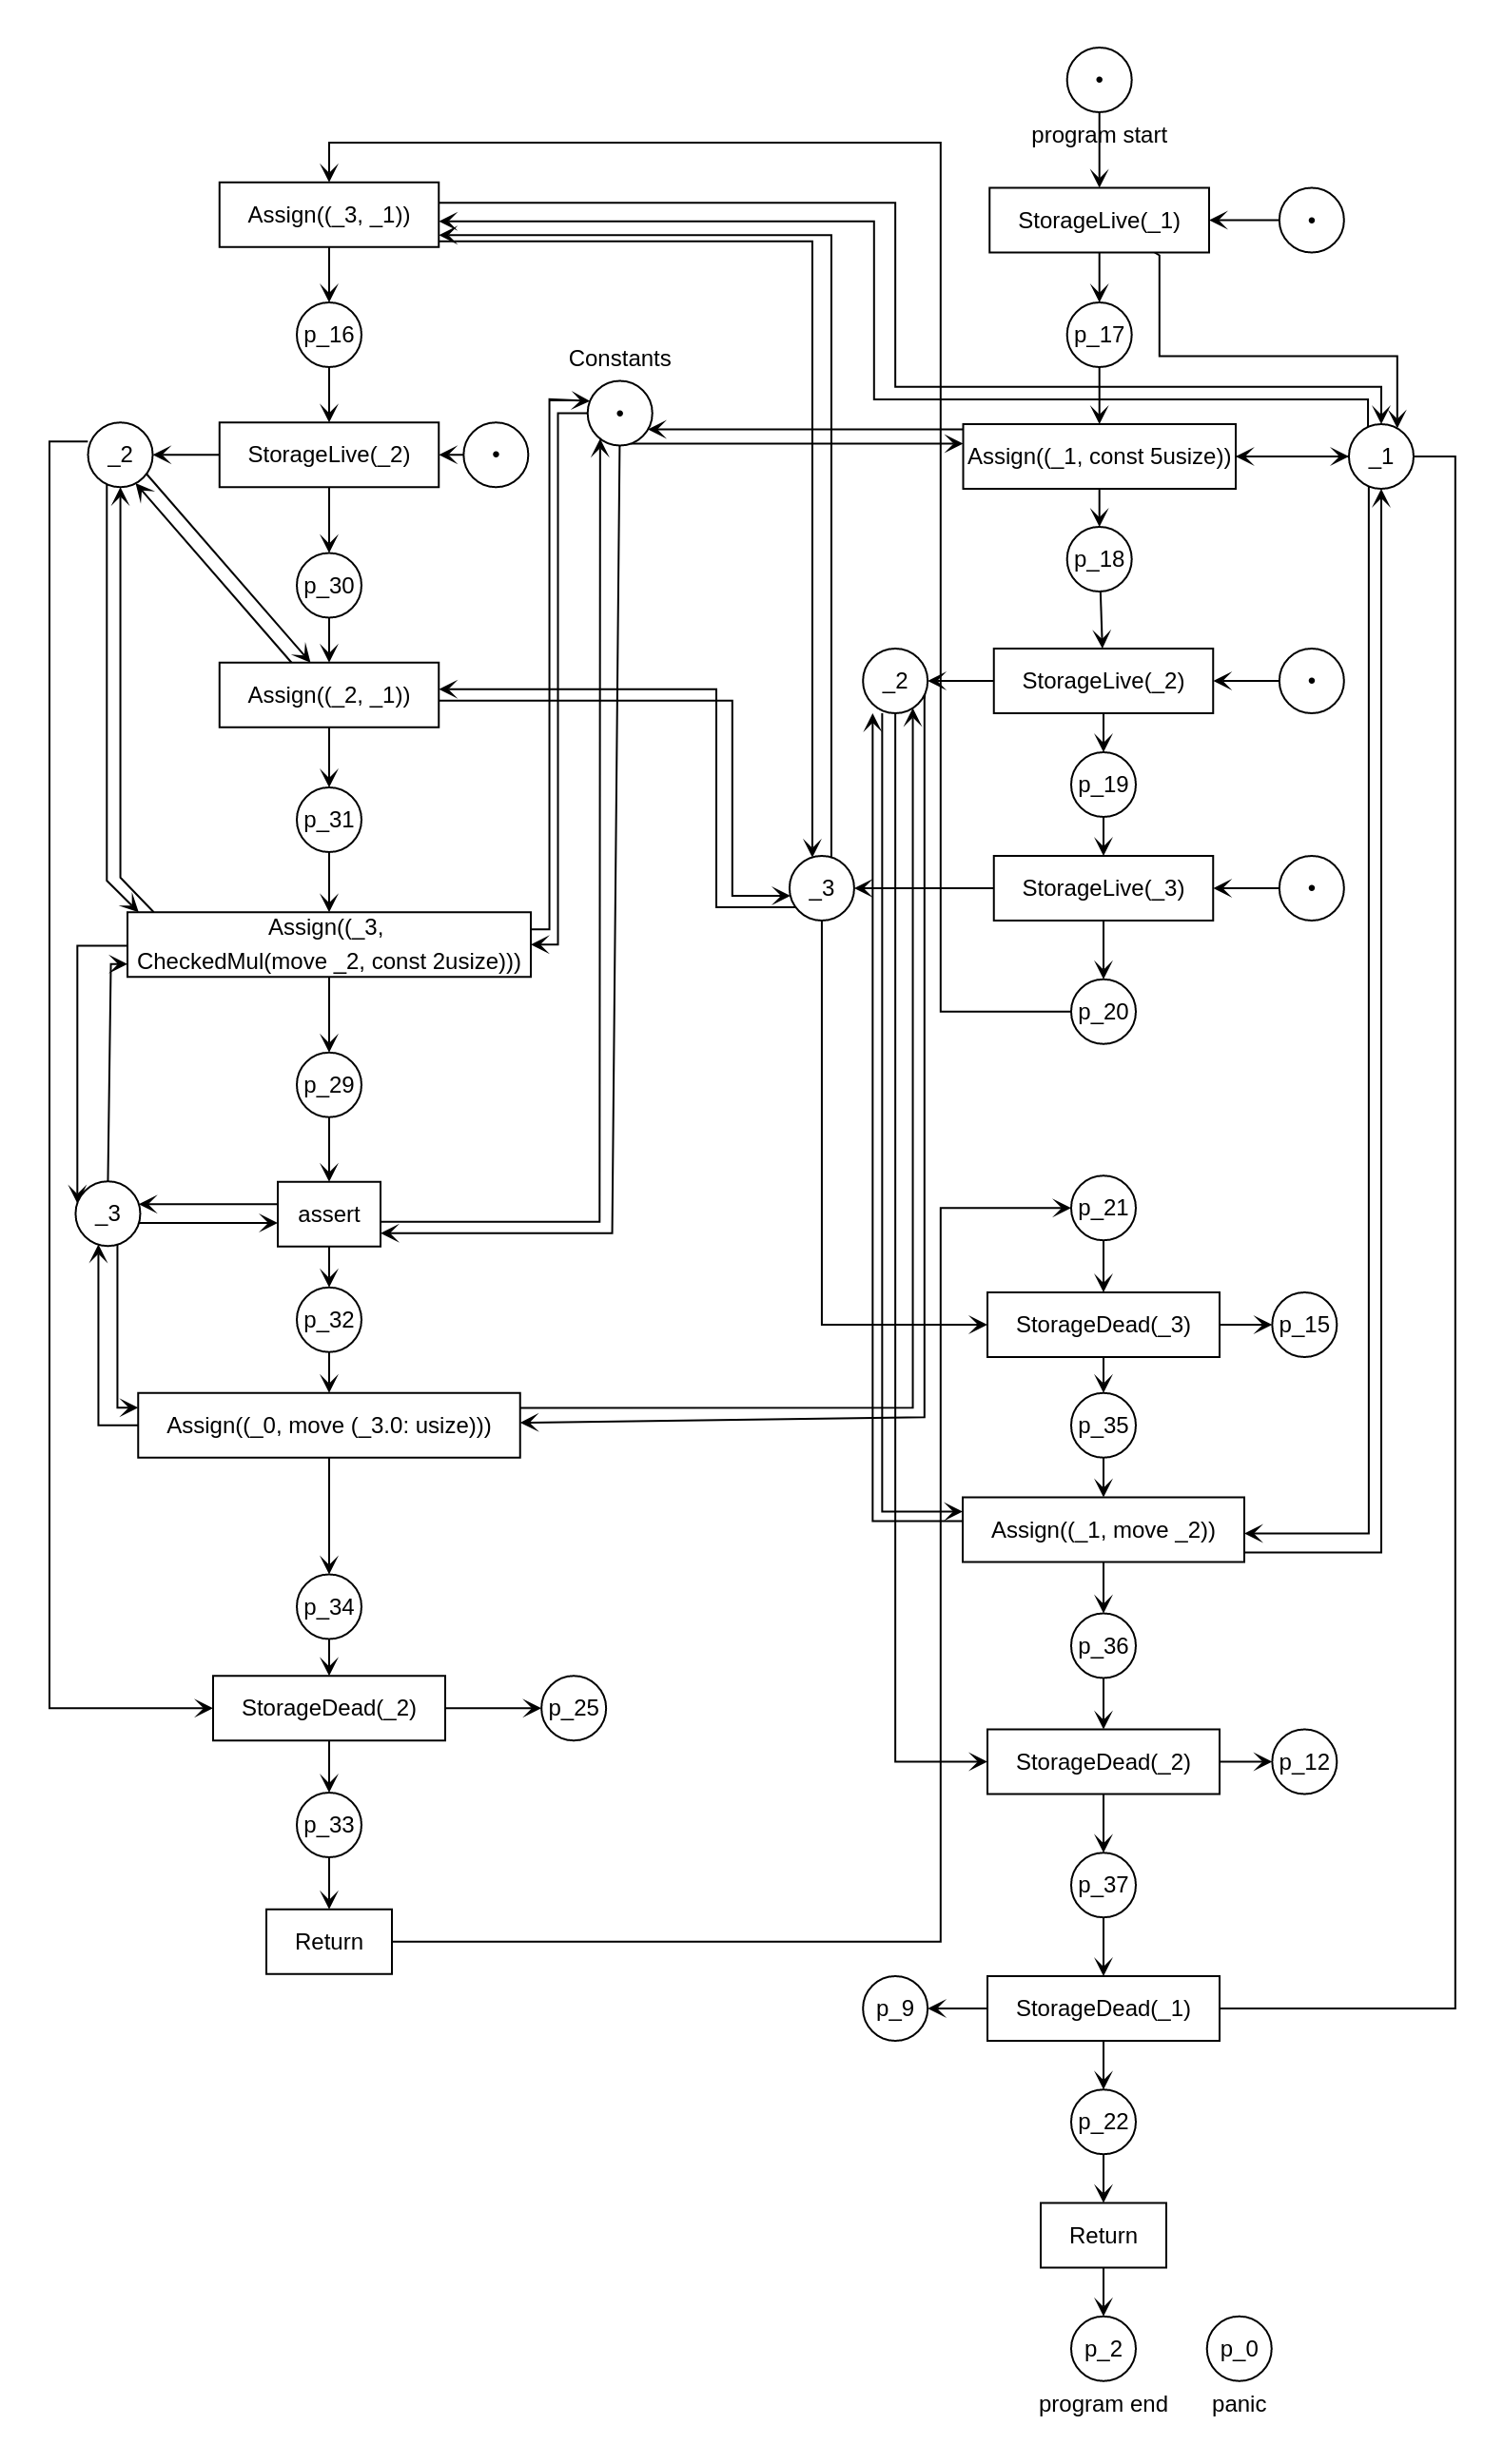
\includegraphics[width=0.9\textwidth]{../diagrams/FunctionCallNet.png}
  \caption{Translated Petr-net}
  \label{function_call_net}
\end{figure}
In figure \ref{function_call_net} we can see the generated net for the function call program \ref{function_call_program} from the last chapter (since this is small enough to show and big enough to not be trivial).
This is the true data that was produced for the dot target so we cannot immediately see the virtual boundaries for statements basic blocks and functions.
To make the structure more clear the nodes where rearranged so that the called function is on the left and the main function on the right.
The initialized places of the locals where renamed to show their MIR name (locals are scoped by functions so their names are not unique).

We can see a path from program start to program end;
The panic place is unconnected because the program cannot panic.
Local life cycles are also visible as a single edged path from marked uninitialized place to unmarked dead places.
Variable manipulation always has parallel incoming and outgoing edges.
On a closer look we can see that local $\_3$ of the called function has no storage live and dead statements.
This is actually a correct representation of the MIR graph:
for some reason the storage statements are not generated for some lvalues (in this case the lvalue from checked multiplications).
If this is expected behavior is not known at the time of writing;
A bug report \cite has yet to be solved.
Unfortunately this behavior introduces an unintended deadlock into our translation since depending transitions can only fire if the initialized places where previously marked.
To use the net for verification we have to work around this issue until it is fixed (or until the cause is modeled correctly).
Te be able to continue testing simply all initialized place where marked.
This way the involved transitions can fire, but only if the previous transition produced a token on the connecting place (the program counter place). 
An additional token will also remain on the initialized places even after the storage dead transition fired.
However execution flow, again, will not be affected because of the program counter places.

A second detail that the net shows is that the function call transition is implicit;
The last statement of the main functions first basic block is directly connected to the first statement of the callees first basic block.
This is an implementation detail of the translator.
Since our model currently always inlines function calls (it generates a separate net for every call), these are entirely sequential.
That means a missing transition does not harm.
If previously translated functions shall be reused though, this issue needs rework.
But to be able to skip inlining we need high level semantics anyway.

An additional issue that can come to attention is the missing cleanup path of the assert terminator.
This is the path that would lead to a panic.
Logically the assert is inserted because the preceding checked multiplication can overflow, which is undefined behavior and by default should panic in Rust semantics.
This particular program cannot fail at this point, since the involved variables are constant and small enough to be multiplied.
If this is the reason why the panic path is not generated (or optimized away) in the MIR representation however, shall be a question for the Rust compiler team.

\section{Verification results}
\begin{figure}
  \centering
  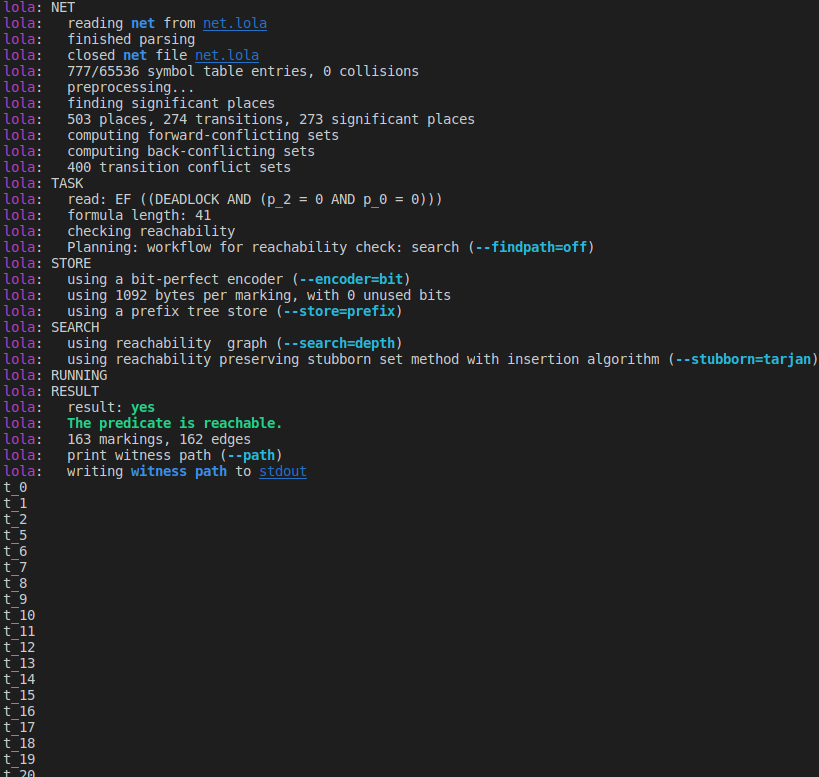
\includegraphics[width=1\textwidth]{./pictures/lola_output.png}
  \caption{LoLa output}
  \label{lola_output}
\end{figure}
Of course we want to use our translation further for verification.
Using our formula on the deadlock program from listing \ref{deadlock_program}, LoLa does find a deadlock and can produce a witness path as shown in figure \ref{lola_output}.
In contrast, if we remove the last line of the program, no deadlock is detected.
Following the witness path in the deadlock case, does indeed lead to the transitions that are involved in the mutex emulation (the mutex place is empty causing involved transitions to be dead).
Earlier tests have also shown that the mutex emulation discussed in chapter \ref{emulation} is necessary to produce deadlocks.
Without the information on where and how execution should be blocked, the translation process cannot infer this behavior.
This is a general problem for blocking behavior by external cause.

At this point it might be adequate to add that active waiting (looping until a guard has an expected value) is not a deadlock and also would not be detected with this approach.
However, it is likely that another formula can be found that verifies that leaving the waiting section is always possible.
But again this most likely would require to consider the values that variables can hold and therefore high-level semantics.

\section{Discussion}
The results show that our basic approach can be used to verify some basic properties.
And even though the state of the translation is nowhere near productive use there are still some lessons that can be learned that we can discuss.
\subsection{The Model}
The main draw back that followed us for the entire process is the abstraction of data in low-level petri nets.
The advantages of the low-level model not only are the reduced complexity and higher verification performance, it can also produce stricter assertions.
Additionally, our particular model most likely can exploit a petri-net property called safety.
If we overlook the workaround for compensating the missing storage-statements, the token count on every place cannot exceed a maximum of one.
One obvious use for that property is the state encoding for every place, which can be done with a single bit this way.
This might be helpful for very large programs with lots of places.

The greatest disadvantage of low level Petri-Nets is the reduced expressivness of data.
While flow related properties are easy to model with simple tokens, as soon as we enter the realm of data related properties, we have to make compromises.
The approach we took models every interaction with data but we cannot facilitate their set of possible values for verification tasks.
Another problem is that no moving data is modeled.
If a previously initialized local becomes part of another local (like a field of a struct) we completely loose this information in our translation.
Although, we can probably exploit Rusts strict borrow checking and aliasing rules to model a much closer relation between data,
both locals are generated independently with their own places and life cycle.
An improvement for example for a move of a value from one local to another (which is encoded in MIR), is to connect the places with a transition right away.

Another disadvantage of our current model is the inlining of functions.
If a program calls the same function at different places, a separat instance will be inserted at every call site.
This not only makes the net larger, it also causes the translation to diverge in recursive functions.

A solution for most of these problems might be high-level Petri-Nets where we can model data verbosely.
With them we could properly model data and detach function calls from the call site.
Only the cost for verification performance remains unknown at the moment.
Some problems, on the other hand, cannot be solved this way.
For example, program parts that are not represented by MIR (like foreign functions and compiler intrinsics) cannot be translated and have to be emulated.
Also information on blocking behavior is needed to model deadlocks appropriately.
For mutexes we again worked around this issue with emulation.
Additional blocking functionality (like waiting threads) have to be emulated separately.

\subsection{Verification}
The ability to discover deadlocks is already a useful property for model checking.
But our model is not restricted to this single property.
An easy addition is to check if the panic state is reachable.
Since increased complexity also increase the likelihood of operation that can panic this might be of limited use;
Unless variable data can be respected.
However, more complex properties could deal with conditional reachability.
For example if a function can be reached from a particular program state.
Or if every execution of a program eventually visits a function or statement.
But then again, our statements would be much stronger if we could consider data values.
